\chapter{Random Sequences and Visualization}\label{ch:randomseq}
%!TEX root = main.tex

Now that we understand the rules of probability, and how they are applied in a number of practical examples, we explore the use of these rules to \emph{sequences of random events}.  This will produce several interesting and unintuitive observations and failures of inference, and the proper ways to handle them.  Finally, we examine how visualize both data in general and what we can communicate with such visualization.

\section{Coin Flipping}

We'll start with some simple examples of coin flipping, asking some simple questions, and move to more complex observations and unintuitive conclusions.

\example{
What is the probability of flipping three heads in a row, with a fair coin?
}

We can approach this problem in two different ways.  The first way, is a brute-force counting method with the definition of probability for exclusive events (using Equation~\ref{eq:p_mutually_exclusive}) and the second way makes use of the other rules of probability.  In the first way, we simply outline every possible combination of three flips, see how many are ``three heads in a row''

\marginnote{
All possible results from three coin flips:

\begin{tabular}{cc}
1 & T T T  \\
2 & T T H  \\ 
3 & T H T   \\
4 & T H H   \\
5 & H T T \\
6 & H T H \\
7 & H H T \\
8 & H H H 
\end{tabular}
}

Because there is only one case of ``H H H'' in all eight, the probability of three heads in a row is
\beqn
\P{three heads in a row}=1/8
\eeqn
which is an unlikely outcome, but not extremely so (see Table~\ref{table1}).


In terms of the rule of probability, we have 
\beqn
\P{three heads in a row}=P(H_{1} \mbox{\bf\ and } H_{2} \mbox{\bf\ and } H_{3})
\eeqn
where $H_{1}$ is heads on the first flip, $H_{2}$ is heads on the second flip, etc...  Because these are {\em independent events} (Section~\ref{sec:independence}), the probability is just the product of the probabilities of the individual events (Equation~\ref{eq:indepprod})
\beqn
\P{three heads in a row}&=&P(H_{1} \mbox{\bf\ and } H_{2} \mbox{\bf\ and } H_{3})\\
&=&P(H_{1})\times P(H_{2})\times P(H_{3})\\
&=&\frac{1}{2}\times\frac{1}{2}\times\frac{1}{2}\\
&=&\frac{1}{8}
\eeqn
the same answer as before.\marginnote{Yet again, we see that if there are multiple ways of arriving at an answer, that it must yield the same answer - equivalent states of knowledge yield equivalent probability assignments.}

\example{
What is the probability of flipping {\em thirty} heads in a row, with a fair coin?
}

Our intuition will clearly insist that this will be a very small number, but how small?  Our first method, of listing all of the possibilities gets quite a bit cumbersome with this question.  The second method is quite straightforward
\beqn
\P{thirty heads in a row}&=&P(H_{1} \mbox{\bf\ and } H_{2} \mbox{\bf\ and } \cdots \mbox{\bf\ and } H_{30})\\
&=&P(H_{1})\times P(H_{2})\times \cdots \times P(H_{30})\\
&=&\overbrace{\frac{1}{2}\times\frac{1}{2}\times\cdots \times \frac{1}{2}}^{\mbox{30 times}}\\
&=&\left(\frac{1}{2}\right)^{30}\\
&=&0.000000001 \mbox{ (one in a billion!)}
\eeqn
This is virtually impossible (Table~\ref{table1}).
\example{
What is the probability of flipping two heads in three flips, with a fair coin?
}

Our intuition suggests that this should be a reasonably common occurrence.  We address this problem in exactly the same two ways: first, by counting, the second with the rules of probability.  In the first method, we observe from the table that there are three ways of getting two heads: ``T H H,'' ``H T H,'' and ``H H T.''  Thus, 
\beqn
\P{two heads in three flips} = \frac{3}{8}
\eeqn
In the second method we write
\beqn
\lefteqn{\P{two heads in three flips}=}\\
&& P\left( (T_{1} \mbox{\bf\ and } H_{2} \mbox{\bf\ and } H_{3})  \mbox{\bf\ or } (H_{1} \mbox{\bf\ and } T_{2} \mbox{\bf\ and } H_{3})  \mbox{\bf\ or } (H_{1} \mbox{\bf\ and } H_{2} \mbox{\bf\ and } T_{3}) \right)
\eeqn
from which we can apply the sum rule for exclusive events (Equation~\ref{eq:exclusive_sum}) and, like before, the product rule for independent events (Equation~\ref{eq:indepprod}),

\beqn
\lefteqn{\P{two heads in three flips}=}\\
&& P(T_{1} \mbox{\bf\ and } H_{2} \mbox{\bf\ and } H_{3})+P(H_{1} \mbox{\bf\ and } T_{2} \mbox{\bf\ and } H_{3})+P(H_{1} \mbox{\bf\ and } H_{2} \mbox{\bf\ and } T_{3})\\
&=&\left(\frac{1}{2}\times\frac{1}{2}\times\frac{1}{2}\right)+\left(\frac{1}{2}\times\frac{1}{2}\times\frac{1}{2}\right)+\left(\frac{1}{2}\times\frac{1}{2}\times\frac{1}{2}\right)\\
&=&\frac{1}{8}+\frac{1}{8}+\frac{1}{8}=\frac{3}{8}
\eeqn
which is about a 38\% chance, slightly unlikely (Table~\ref{table1}).

\example{
What is the probability of flipping ten heads in thirty flips, with a fair coin?
}

Once the numbers start getting large, our intuition fails, and we can't list all the possibilities.  In order to proceed, we need to develop a systematic way of approaching these sorts of problems.  Essentially it comes down to two parts:
\be
\i What is the probability of {\em one particular sequence} being considered?
\i How many ways can this {\em type of sequence} appear in the process described in the question?
\ee

Point 1 is asking, what is the probability of this particular sequence:
\begin{center}
H H H H H H H H H H T T T T T T T T T T T T T T T T T T T T 
\end{center}
or this sequence:
\begin{center}
T T H T T T T H H H H T T T T T H T T H T T T T T T H H T H
\end{center}
Although it is unintuitive, mathematically both of these specific sequences have {\em exactly} the same probability: each head or tail has equal probability, is not related to the others, and there are the same number of them.  So we have
\beqn
\lefteqn{\P{HHHHHHHHHHTTTTTTTTTTTTTTTTTTTT}=}\\
&&\P{TTHTTTTHHHHTTTTTHTTHTTTTTTHHTH}\\
&=&\left(\frac{1}{2}\right)^{30}\\
&=&0.000000001 \mbox{ (one in a billion!)}
\eeqn
Every single specific length-thirty sequence of heads and tails has the same probability, one in a billion.

Point 2 is asking, how many sequences are there of thirty heads and tails where ten of them are heads?  Another way of phrasing it is, given a sequence like:
\begin{center}
H H H H H H H H H H T T T T T T T T T T T T T T T T T T T T 
\end{center}
how many different ways can I rearrange this sequence and get a unique sequence?

\subsection{Counting the Rearrangements}

We are going to determine the answer to our question in small steps.  \marginnote{
Symbols: A B C D
}

\marginnote{
Boxes: \raisebox{.03in}{\framebox[.1in]{\ } \framebox[.1in]{\ } \framebox[.1in]{\ } \framebox[.1in]{\ }}
}
\marginnote{
\begin{tabular}{cc}\\
Choices& Remaining Symbols\\\hline\hline
A \raisebox{.03in}{\framebox[.1in]{\ } \framebox[.1in]{\ } \framebox[.1in]{\ }} & B C D \\
B \raisebox{.03in}{\framebox[.1in]{\ } \framebox[.1in]{\ } \framebox[.1in]{\ }} & A C D \\
C \raisebox{.03in}{\framebox[.1in]{\ } \framebox[.1in]{\ } \framebox[.1in]{\ }} & A B D \\
D \raisebox{.03in}{\framebox[.1in]{\ } \framebox[.1in]{\ } \framebox[.1in]{\ }} & A B C
\end{tabular}

}
First, we ask, 
\example{
How many ways can we rearrange the unique symbols A, B, C, and D?
}
To make this intuitive, we set up four empty boxes
and we imagine placing our symbols in the boxes, one at a time.  How many choices do we have?  For the first box, we have four choices.  For each of these choices, we've removed one of the symbols, and one of the boxes.  \marginnote{
\begin{tabular}{cc}\\
Choices& Remaining Symbols\\\hline\hline
A B \raisebox{.03in}{\framebox[.1in]{\ } \framebox[.1in]{\ }} & C D \\
A C \raisebox{.03in}{\framebox[.1in]{\ } \framebox[.1in]{\ }} & B D \\
A D \raisebox{.03in}{\framebox[.1in]{\ } \framebox[.1in]{\ }} & B C \\
& \\
B A \raisebox{.03in}{\framebox[.1in]{\ } \framebox[.1in]{\ }} & C D \\
B C \raisebox{.03in}{\framebox[.1in]{\ } \framebox[.1in]{\ }} & A D \\
B D \raisebox{.03in}{\framebox[.1in]{\ } \framebox[.1in]{\ }} & A C \\
& \\
C A \raisebox{.03in}{\framebox[.1in]{\ } \framebox[.1in]{\ }} & B D \\
C B \raisebox{.03in}{\framebox[.1in]{\ } \framebox[.1in]{\ }} & A D \\
C D \raisebox{.03in}{\framebox[.1in]{\ } \framebox[.1in]{\ }} & A B \\
& \\
D A \raisebox{.03in}{\framebox[.1in]{\ } \framebox[.1in]{\ }} & B C \\
D B \raisebox{.03in}{\framebox[.1in]{\ } \framebox[.1in]{\ }} & A C \\
D C \raisebox{.03in}{\framebox[.1in]{\ } \framebox[.1in]{\ }} & A B 
\end{tabular}

}
Thus, we are left with three remaining symbols for each choice, and three remaining boxes. For each of the original four choices, we now have three choices for the second box.  This immediately leads to $4\times 3=12$ possibilities by the time we've filled two boxes.  For each of these twelve possibilities, there are two symbols remaining and two boxes.  Continuing this logic, we have two choices for the third box, and then only one choice for the final box.  In summary, for each of the four choices for the first box we have three choices for the second, two choices for the third, and one for the final box.  Thus we have
\beqn
\left(\parbox{1.6in}{number of rearrangements of four different symbols}\right)=4\times 3 \times 2 \times 1 = 24
\eeqn
In general we have
\highlight{Number of Rearrangements of $N$ Unique Symbols}{
\beq
\nn C(N)&=&N\times (N-1) \times \cdots \times 2 \times 1 \\
&=&N! \label{eq:rearrangements_unique}
\eeq
where we've introduced the notation for the {\em factorial of $N$} as $N!$.
}{
\beqn
C(N)&=&N\times (N-1) \times \cdots \times 2 \times 1 \\
&=&N!
\eeqn
}

\example{
How many ways can we rearrange the symbols A, A, A, and D?
}
\marginnote{
Symbols: A A A D
}
\marginnote{
\begin{tabular}{c}
Rearrangements \\ \hline\hline
D A A A \\
A D A A \\
A A D A \\
A A A D
\end{tabular}
}

By eye we can see that there are only four rearrangements of these symbols.  How is this different from the previous question with four symbols?  We can imagine going from the first question, with four unique symbols ``A B C D,'' and replace both ``B'' and ``C'' with ``A'' to get it.   ``BC'' and ``CB'' are different sequences of unique symbols.  However, if we replace ``B'' with an ``A'' and ``C'' with an ``A'', both sequences become the same sequence, namely ``AA''.  If we try to blindly apply Equation~\ref{eq:rearrangements_unique}, the one for the number of rearrangements of {\em unique} symbols, to the case where there are duplicates, we will {\em overestimate} the number of rearrangements - we are over counting duplicate subsequences.  Further, we can be specific about how much we are over counting and thus find a new equation which includes the possibility of duplicates.

For example, if we have three duplicates in a sequence, the number of over countings will be the number of possible rearrangements of three unique symbols, because all of these rearrangements result in the same sequence of duplicate symbols.  Thus, our procedure should be, 
\beqn
\left(\parbox{1.2in}{number of rearrangements of ``A A A D''}\right)&=&\frac{\left(\parbox{1.6in}{number of rearrangements of four \emph{unique} symbols}\right)}{\left(\parbox{1.6in}{number of rearrangements of the over-counted duplicate three symbols}\right)}\\
&=&\frac{4!}{3!} \\
&=&\frac{4\times 3 \times 2 \times 1}{3 \times 2 \times 1}\\
&=&4
\eeqn

\example{
How many ways are there of rearranging the symbols ``A A A D D''?
}

Following the same logic, we have
\beqn
\overbrace{\underbrace{\mbox{A A A }}_{\parbox{.8in}{$3!$ ways of rearranging 3 duplicates}}\underbrace{\mbox{D D}}_{\parbox{.8in}{$2!$ ways of rearranging 2 duplicates}}}^{\parbox{.8in}{$5!$ ways of rearranging 5 \emph{unique} symbols}}
\eeqn

\marginnote{
All possible results of rearranging the symbols ``A A A D D'':

\begin{tabular}{cc}
1 & A A D D A \\
2 & D A A D A \\
3 & A D A D A \\
4 & D A A A D \\
5 & D A D A A \\
6 & A A D A D \\
7 & D D A A A \\
8 & A D D A A \\
9 & A A A D D \\
10 & A D A A D
\end{tabular}
}

\beqn
\left(\parbox{1in}{number of rearrangements of ``A A A D D''}\right)&=&\frac{5!}{3!2!} \\
&=&\frac{5\times 4 \times 3 \times 2 \times 1}{(3 \times 2 \times 1) \times (2 \times 1)}\\
&=&\frac{120}{6\times 2} \\
&=&10
\eeqn

\subsection{Sequences of Heads and Tails}

Now we can return to our original question, 
\example{
What is the probability of flipping ten heads in thirty flips, with a fair coin?
}

We broke it down into two parts:

\beqn
P(h=10,N=30) = \P{\parbox{1in}{one sequence of 10 heads and 20 tails}} \times \left(\parbox{1in}{number of rearrangements of a length-30 sequence with 10 ``H'' and 20 ``T''}\right)
\eeqn

\be
\i What is the probability of {\em one particular sequence} being considered?

\beqn
\P{\parbox{1in}{one sequence of 10 heads and 20 tails}}&=&\left(\frac{1}{2}\right)^{10}\times \left(\frac{1}{2}\right)^{20} \\
&=&\left(\frac{1}{2}\right)^{30} \\
&=&0.00000000093 \mbox{ (one in a billion!)}
\eeqn

\i How many ways can this {\em type of sequence} appear in the process described in the question?

Because we have a length-thirty sequence of ``H'' and ``T'' with 10 duplicate ``H'' symbols and 20 duplicate ``T,''  we have the following number of ways that this could occur (i.e. the number of rearrangements of these sequences):
\beqn
\left(\parbox{1in}{number of rearrangements of a length-30 sequence with 10 ``H'' and 20 ``T''}\right)&=&\frac{30!}{10!20!} \\
&=&30045015
\eeqn
\ee

So the probability of flipping 10 heads in 30 flips is 
\beqn
P(h=10,N=30)&=&\frac{30!}{10!20!}\left(\frac{1}{2}\right)^{30}\\
&=&30045015\times 0.00000000093 \\
&=&0.028
\eeqn
which is extremely unlikely (Table~\ref{table1}).  

In general we have
\highlight{Probability of flipping $h$ heads and $t$ tails}{
Given the probability of flipping a single heads as 1/2, and the total number of flips is $N=h+t$, we have the following equivalent forms:
\beq
P(h,t)&=&\frac{(h+t)!}{h!t!}\times \left(\frac{1}{2}\right)^{h}\times \left(\frac{1}{2}\right)^{t}\\\label{eq:prob_heads}
\nn P(h,N)&=&\frac{N!}{h!(N-h)!}\times \left(\frac{1}{2}\right)^{h}\times \left(\frac{1}{2}\right)^{N-h} \\
\nn P(h,N)&=&\nchoosek{N}{h}\times \left(\frac{1}{2}\right)^{h}\times \left(\frac{1}{2}\right)^{N-h}
\eeq
where we have introduced the notation that is sometimes used, called {\em choose}, read as ``N choose h,''
\beqn
\nchoosek{N}{h}&\equiv&\frac{N!}{h!(N-h)!}
\eeqn
}{
Given the probability of flipping a single heads as 1/2, and the total number of flips is $N=h+t$, we have the following probability for $h$ heads and $t$ tails:
\beqn
P(h,t)=\frac{(h+t)!}{h!t!}\times \left(\frac{1}{2}\right)^{h}\times \left(\frac{1}{2}\right)^{t}
\eeqn
} 

Shown in Figure~\ref{fig:coinflips1} is the probability of flipping $h$ heads in 30 flips, for each value of $h$ from $h=0$ (no heads or, in other words, 30 tails) up to $h=30$ (all 30 heads). Clearly the most likely value is 15, but all of the numbers from 12 up to 18 have significant probability.

\begin{figure}
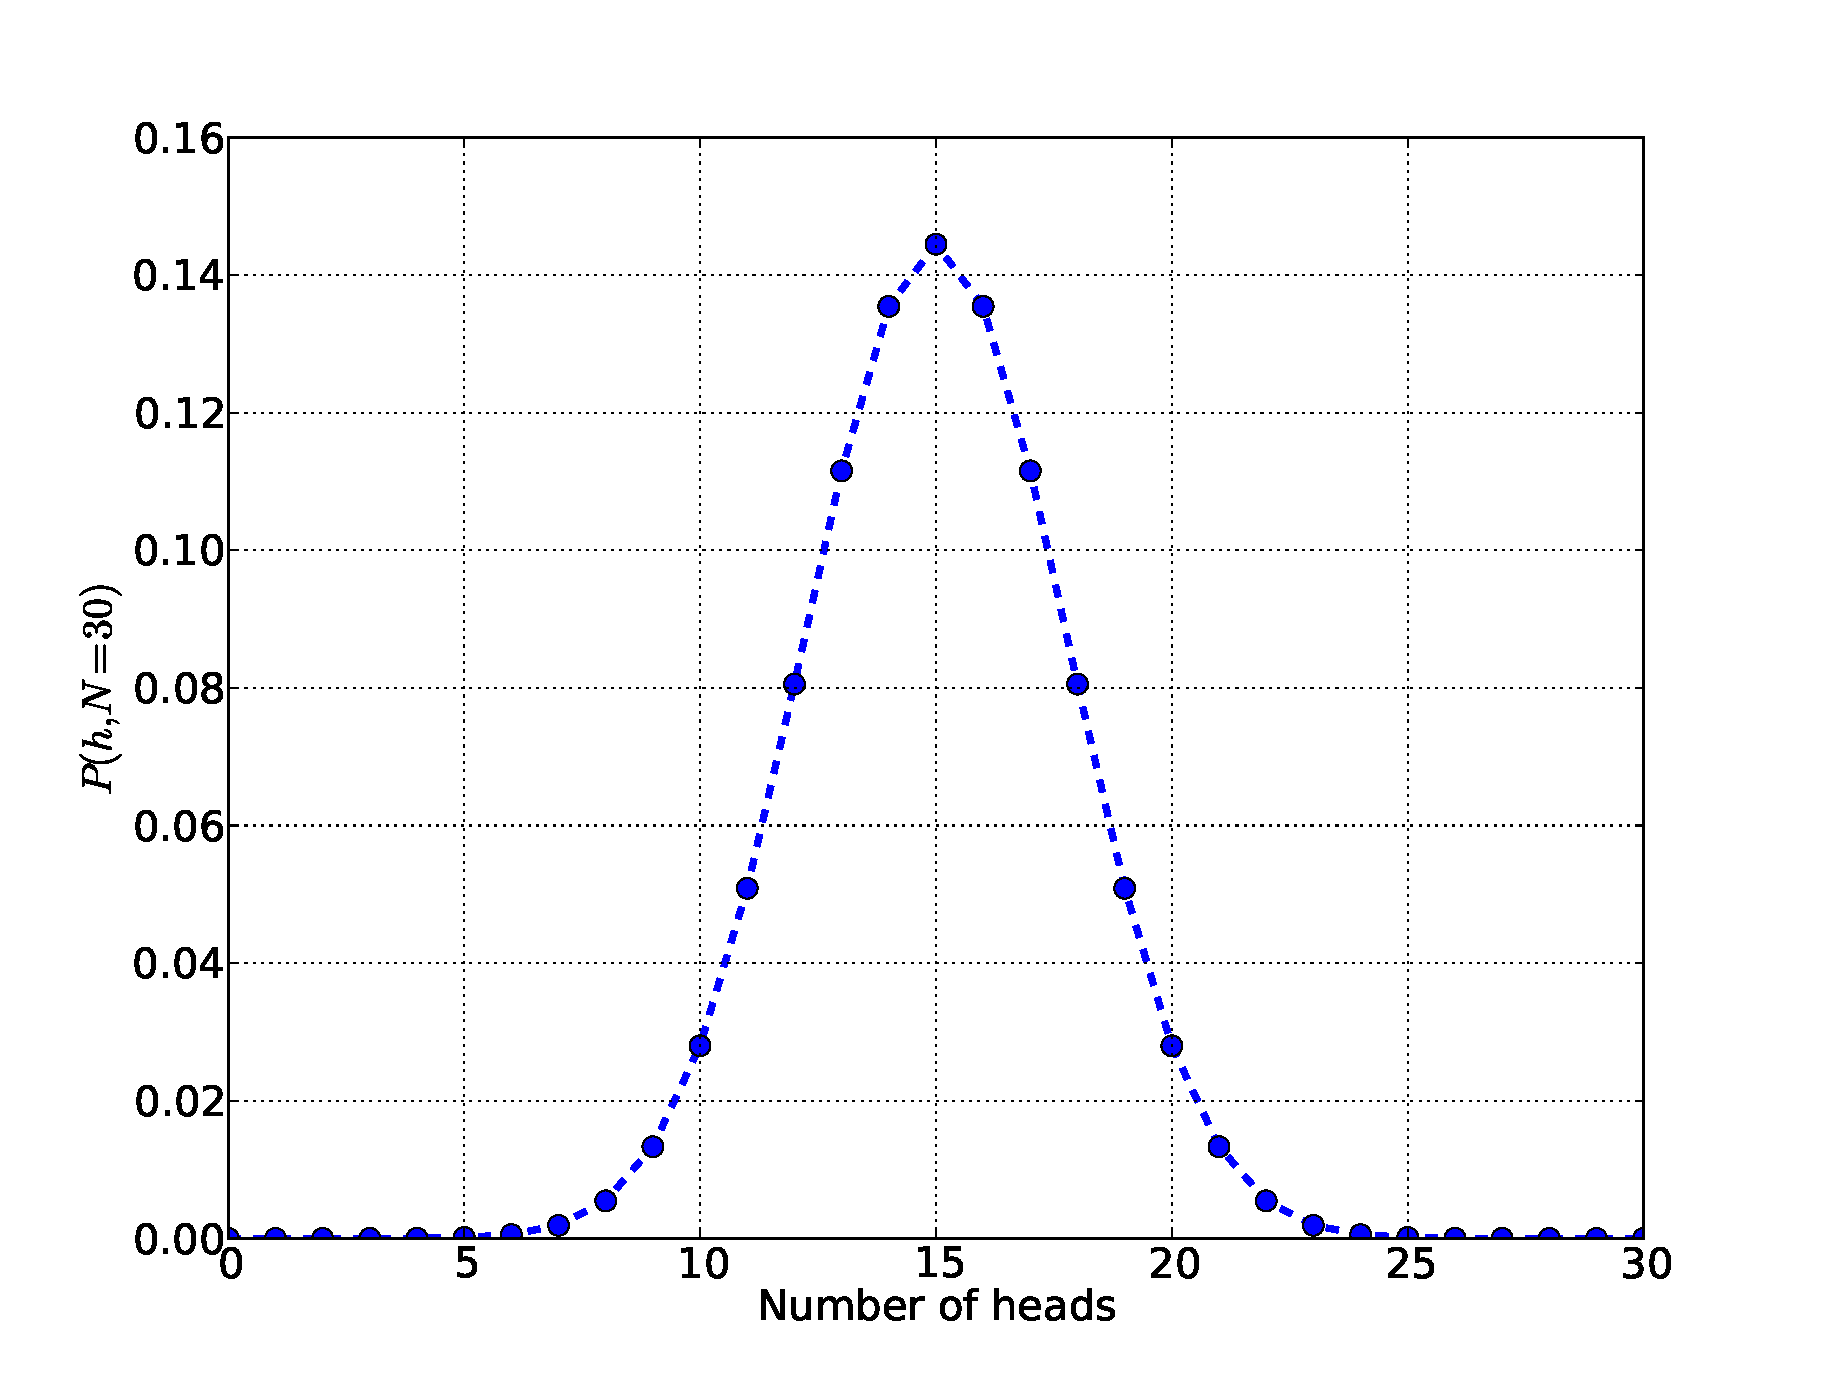
\includegraphics{coinflips1}
\label{fig:coinflips1}
\caption{Probability of getting $h$ heads in 30 flips.  Clearly the most likely value is 15, but all of the numbers from 12 up to 18 have significant probability.}
\end{figure}

\example{What is the probability of getting 17 or more heads in 30 flips?}

Because these are independent events, we can simply sum up the terms for $P(h=17,N=30)$, $P(h=18,N=30)$, etc... yielding the following, either through direct calculation, or by reading the Figure~\ref{fig:coinflips1}.

\beqn
P(h\ge 17,N=30)&=&\underbrace{0.11}_{h=17} + \underbrace{0.08}_{h=18} + \underbrace{0.05}_{h=19} + \underbrace{0.028}_{h=20} + \underbrace{0.013}_{h=21} + \underbrace{0.005}_{h=22} + \underbrace{0.002}_{h=23} + \underbrace{\mbox{(tiny numbers)}}_{h=23, 24, 25, 26, 27, 28, 29, 30} \\
=0.29
\eeqn
which is quite likely!


\section{Binomial Distribution}

The distribution of the possible number of \emph{heads}, given $N$ flips with a coin with probability $p$ of flipping heads, is referred to as the Binomial Distribution.  It has the form of Equation~\ref{eq:prob_heads}, with the ``fair coin'' probability, $1/2$, replaced with $p$:
\beq
P(h|N,p)&=&\frac{N!}{h!(N-h)!}\times p^{h}\times (1-p)^{N-h}\label{eq:binomial}
\eeq


\highlight{Probability of flipping $h$ heads and $t$ tails with an {\em unfair} coin}{
Given the probability of flipping a single heads is, say, $p$ and the total number of flips is $N=h+t$, we have the following equivalent forms:
\beq
P(h,t)&=&\frac{(h+t)!}{h!t!}\times p^{h}\times (1-p)^{t}\\
\nn P(h,N)&=&\frac{N!}{h!(N-h)!}\times p^{h}\times (1-p)^{N-h} \\
\nn P(h,N)&=&\nchoosek{N}{h}\times p^{h}\times (1-p)^{N-h}
\eeq
where the probability of tails is $1-p$.
}{
Given the probability of flipping a single heads as $p$, and the total number of flips is $N=h+t$, we have the following probability for $h$ heads and $t$ tails:
\beqn
P(h,t)=\frac{(h+t)!}{h!t!}\times p^{h}\times (1-p)^{t}
\eeqn
} 

\begin{figure}
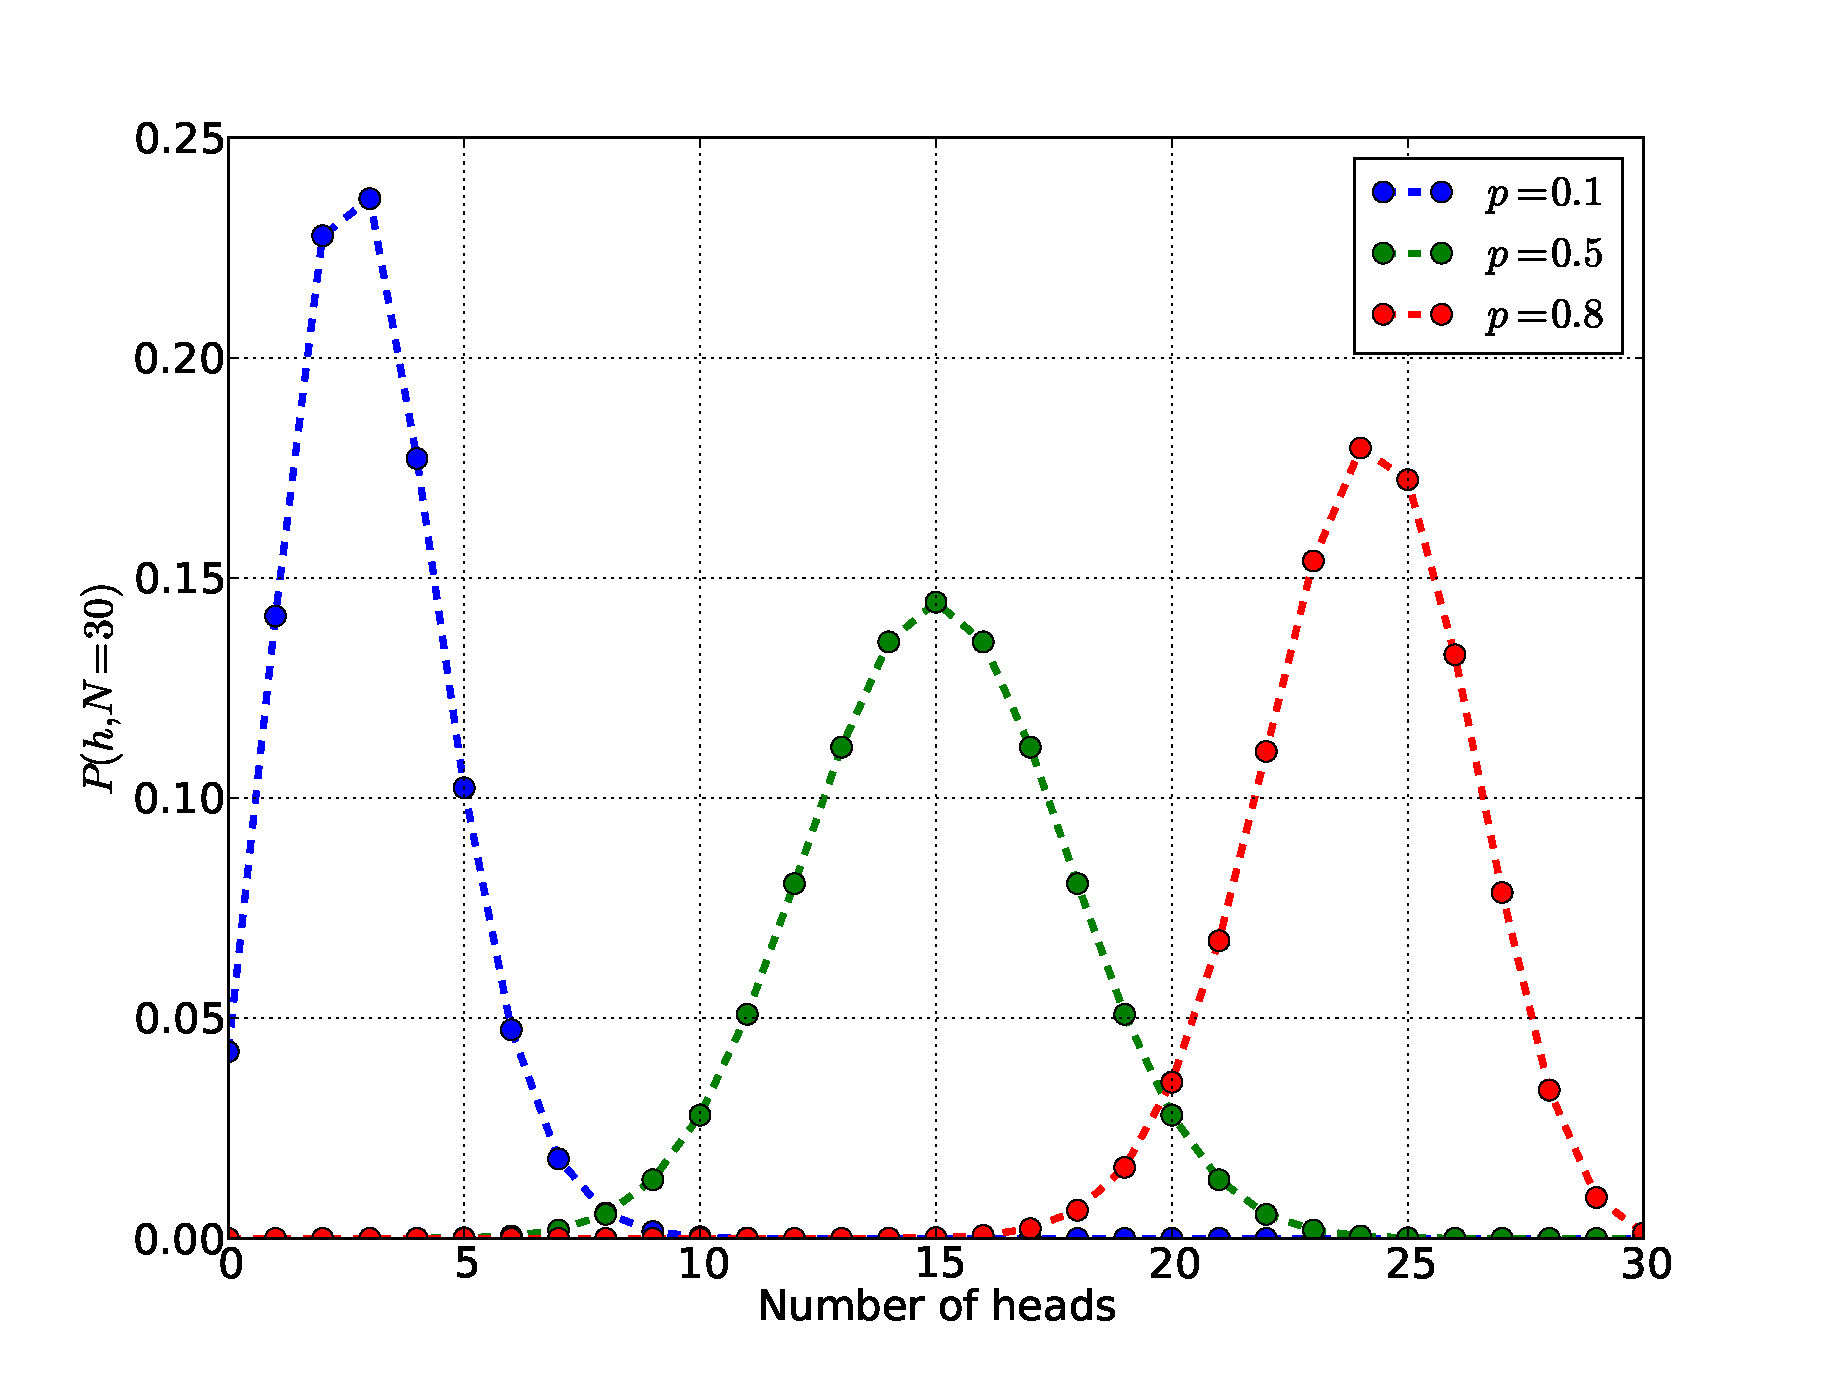
\includegraphics{coinflips5}
\label{fig:coinflips5}
\caption{Probability of getting $h$ heads in 30 flips given a possible unfair coin. One coin has $p=0.1$, where the maximum is for 3 heads (or 1/10 of the 30 flips), but 2 heads is nearly as likely.  Another has $p=0.5$, and is the fair coin considered earlier with a maximum at 15 heads (or 1/2 of the 30 flips).  Finally, another coin shown as $p=0.8$ where 24 heads (or 8/10 of the 30 flips) is maximum. }
\end{figure}




\section{Streaks}

In the previous section we looked at the probability of getting a certain number of heads in a number of flips.  Look at the following two sequences:
\be
\i HTTHTHHTTHTHTTHHHTHHTTHHTHHTTHTHHTHHTTHTTHHHTHTHTT
\i HHTHHHTTTTTTTHTHTTHTTTHTHTHHTHTTHTTTHHTTTHHHHTHHHH
\ee
One of these sequences was generated from actually flipping a coin 50 times.  The other one is from a person {\em pretending} to flip a coin, and writing down a sequence that they thought would look like a random flipping of a coin.  Which one is which?  While many people think that sequence 1 looks more ``random'' (i.e. it seems to flip around a lot), sequence 2 is actually the random sequence.  

One of the truly unintuitive things about real random sequences, as opposed to designed sequences, is that there are long runs or {\em streaks}.  Why is this?  The general solution is beyond this book but we can think about it this way.  Although a sequence of, say, 5 heads in a row is very unlikely ($\P{5 heads in a row}=(1/2)^{5}=0.03$), there are many opportunities for such a sequence {\em somewhere} within a sequence of 50.  Because of these many opportunities, this raises the probability from 3\% (the probability of 5 heads in a row in 5 flips), to over 55\%, the probability of finding 5 heads in a row {\em somewhere} in 50 flips.  Streaks of 6 heads in a row occur nearly one third of the time in 50 flips, or over half the time if you consider a run to be either heads or tails.  Even streaks of 9 heads or tails in a row, in 50 flips, are not extremely unlikely!
\section{Gambler's Fallacy}

When we look at a sequence of real coin flips, like:
\bi
\i HHTHHHTTTTTTT
\ei
and we ask about the probability of flipping heads in the next flip, it is common to (mistakenly!) reason that, because we've seen 7 tails in a row, then the {\em next} flip is more likely to be heads.  However, this is not the case for two reasons:
\be
\i long streaks are common in completely fair and random sequences - so observing a streak of 7 tails does not contribute much to one's confidence that we are looking at a rigged coin or one that has changed its probability properties.
\i the process of flipping a coin is {\em independent} each time, nearly by definition, and thus the result of one flip cannot influence the result of the next flip.\footnote{One can imagine a flipping procedure where the flips are not independent.  Say, you always place the resulting face (heads or tails) {\em initially up} in a flip, and the you do not flip particularly vigorously.  Thus, the result of one flip would be related to the result of the next flip.  However, in nearly all real cases, people go to great lengths to avoid this sort of procedure.}
\ee

The faulty, but intuitive, reasoning goes by the name of the Gambler's Fallacy and appears in many places.  We can ask a question:\begin{quote}
How could we tell the difference between a random, independent sequence and one where the events are not independent, where the next flip depended on a previous flip?
\end{quote}
We'll have to return to this question later, when we consider model comparison, but roughly, one would have to look at all {\em pairs} of events to see if one pair (say heads-tails) occurs more frequently (even if only by a little) than another pair (say heads-heads).  

In a total fit of irony, casino slot machines \emph{do not produce independent winnings} - they are programmed so that if you've lost many times, then that machine is a little less likely to lose the next time.  In effect, at gambling houses they train the gamblers in the Gambler's Fallacy!


\section{The Hot Hand - Correlations in Random Sequences}

Some work by Tversky and Gilovich\cite{tversky2005cold} looks at the following issue in the sport of basketball:  there are times when it seems as if basketball players have a ``hot hand'' - they are on a shooting streak.  Tversky and Gilovich looked at how basketball fans {\em perceived} streaks, by having them rate sequences of shots as {\em random shooting} or {\em streak shooting}.  Most (65\%) of the respondents classified artificially generated, purely random sequences as {\em streak shooting}.  In real data, they discovered that the actual probability of ``making a given shot (i.e. a player's shooting {\em percentage}) is unaffected by the player's prior performance.''  We examine this effect in a later section (see Example~\ref{ex:hothand} on page~\pageref{ex:hothand}) where we explore the quantitative procedure for assessing this conclusion.  It is enough here to note the large difference between the {\em perception} of the sequence and the likely {\em cause} of the sequence, and thus the need to always be vigilant against faulty perceptions.  Tversky and Gilovich insist that ``their observations do not tell us anything general about sports, but it does suggest a generalization about people, namely that they tend to 'detect' patterns even where none exist.''

What we have here, again, is the general perception that {\em long sequences} are somehow not ``random,'' when in fact the opposite is the case.  People have a natural tendency to see patterns in random data, to infer order where there is none, and to ascribe importance to the appearance of pattern.  It is the role of statistical inference in general to provide the tools to properly handle the distinction between random effects and patterns, and to retune our intuitions.

\section{Regression Toward the Mean}
There is a peculiar phenomenon referred to as {\em regression toward the mean}, which often is misinterpreted and leads to failures of proper statistical inference.  It can be seen in a simple example.  Imagine that we ``test'' a number of students by having them guess the results of a coin flip.  Clearly this will be entirely luck, because the coin flip has no pattern.  If a student guesses the results of 50 flips, there will be an expectation of getting 25 correct.   Here we simulate 20 students each ``predicting'' the result of 50 flips, the results shown in Table~\ref{tbl:coinguess}.  The test is done twice, and we will look at a particular subset presently.  One can, by eye, see that most of the students get around 25 correct - exactly as expected from random performance.

\begin{table}
\begin{center}
\begin{tabular}{cp{.8in}p{.8in}}
\toprule
Student& Total Correct First Round& Total Correct Second Round\\
\midrule
1 & 23  & 24 \\
2 & 23  & 29 \\
3 & 19  & 23 \\
4 & 26  & 27 \\
5 & 28  & 29 \\
6 & 26  & 22 \\
7 & 23  & 26 \\
8 & 30  & 28 \\
9 & 24  & 21 \\
10 & 27  & 23 \\
11 & 25  & 31 \\
12 & 30  & 21 \\
13 & 20  & 22 \\
14 & 28  & 29 \\
15 & 24  & 25 \\
16 & 25  & 22 \\
17 & 23  & 24 \\
18 & 20  & 28 \\
19 & 20  & 29 \\
20 & 28  & 25 \\
\bottomrule
\end{tabular}
\end{center}
\caption{Total Correct Guesses from Students ``Predicting'' the Results of 50 Coin Flips.  Shown are the results of a first round and a second round of guessing.}
\label{tbl:coinguess}
\end{table}


\begin{table}
\begin{center}
\begin{tabular}{c||c}
\toprule
&\\
{\bf Top Five the First Time} & {\bf Bottom Five the First Time}\\
\begin{tabular}{cp{1.2in}}\\
Student& Performance the Second Time\\\hline
8 & Worse \\
12 & Worse \\
14 & Better \\
5 & Better \\
20 & Worse 
\end{tabular} &
\begin{tabular}{cp{1.2in}}\\
Student& Performance the Second Time\\\hline
3 & Better \\
13 & Better \\
18 & Better \\
19 & Better \\
1 & Better 
\end{tabular}\\
\bottomrule
\end{tabular}
\end{center}

\caption{Performance in the Second Round of Students ``Predicting'' the Results of 50 Coin Flips.  Shown are the results for those students who performed \emph{best} in the first round (left), and those that performed \emph{worst} in the first round (right). }
\label{tbl:coinguess_second}
\end{table}





Now, imagine that we look at the {\em top five} coin flip predictors on the first round.  Will they do better or worse in the the second round?  What about the {\em bottom five} coin flip predictors?  The results of these two cases are summarized in Table~\ref{tbl:coinguess_second}. The pattern, even in this small sample, is quite clear:
\be
\i Those that did the best the first time did worse the second (on average)
\i Those that did the worst the first time did better the second (on average)
\ee
One might be tempted (had you not known that this is artificial data, and completely random) to interpret this as a causal pattern, e.g. ``the students that did better the first time, grew over-confident the second,'' ``the students that did worse the first time, worked harder to improve the second,'' etc...  This {\em interpretation} of the results by students has been observed in the classroom.\cite{Gelman2002}  However, it runs into serious trouble when the data is something like the heights of children compared to their parents - the tallest parents tend to have children shorter than they are, the shortest parents tend to have children taller than they are, a pattern first quantified by Galton in 1869\cite{galton1914hereditary}.  He noted that clearly the children are not \emph{trying} to be tall, so effort is not a good explanation for the pattern.


What is happening here is that, if the process is dominated by {\em luck} or simple random variation, then outliers occur, but are rare.  Thus a particularly high value will likely be followed by a lower value - closer to the mean.  The tendency is to regress {\em toward the mean} in processes dominated by luck.  This can be confused with the Gambler's Fallacy discussed earlier, where flipping 3 heads in a row doesn't give you any information about flipping another heads - it is {\em not} more likely to be tails.  Part of the difference is that we are dealing with a process that has {\em many possible values}, not just two, and thus we can have a mean value, and outliers.  

When each of these ideas is applied to sports, the weather, or business there are some interesting conclusions.
\be
\i even when the process is {\em entirely random}, long streaks occur - and are often misinterpreted as an increase in the probability of the event.
\i when a person performs very well at their job (a number of successful business decisions, a high batting average, etc...) they will often do {\em worse} the next year - and again many are surprised, and interpret the result as the person ``losing their touch'' - when in fact, they may just have been lucky for a bit, and are now performing closer to their typical average level.
\i when one has a particularly bad winter, it may be more likely that the next winter won't be quite do bad - due entirely to regression to the mean.  It may, however, be part of a larger pattern (e.g. a large-scale climate oscillation, such as El Ni\~{n}o) and the probability of another bad winter might be \emph{higher}.  In order to tell the difference, we need to construct reasonable models of the phenomena, test those models with predictions, and apply those models into the future.  At each step, we need to be careful not to jump to the conclusion of the existence of a pattern too quickly.
\ee


\section{Visualization of Data}

There are two main methods of visualizing data, and several others that are related to these methods.  In this section we introduce just two, histograms and scatter plots, and we will use these throughout the text.

\subsection{Histograms}

Histograms are a way of {\em summarizing} data, when presenting the entire data set is impractical, or where some understanding of the data is made clearer by summarizing.  The histogram plot is done with the following steps:\marginnote{Another advantage to learning to understand how to generate histograms is that it alerts you to the possible {\em abuses} of these plots.  These abuses can be simple mistakes, which end up giving a misleading message, or a deliberate deception.  Either way, a proper understanding of the process helps.}
\be
\i Choose a number of {\em bins} to divide the data.  
\i Count up the data that fall into each bin
\i Make a {\em bar plot}, or a {\em scatter plot} to present the data.
\ee
The following is an example with a small data set.  The process of binning and counting is often done by computer, but it is instructive to perform the process by hand a few times in order to understand what the results are.

Table~\ref{tbl:male_heights} shows a collection of 106 heights (in centimeters) of the male students in a class\cite{Arel-Bundock:2014uq}.  As a collection of numbers it is relatively opaque, but as a histogram it is clearer.

\begin{table}
\begin{center}
\begin{tabular}{cccccc}
\toprule
177.8& 160.0& 165.0& 182.88& 175.0& 167.0\\
182.88& 190.5& 177.0& 190.5& 180.34& 180.34\\
184.0& 172.72& 175.26& 167.0& 180.0& 180.0\\
190.0& 182.5& 185.0& 171.0& 172.0& 180.34\\
180.0& 170.0& 200.0& 190.0& 170.18& 179.0\\
182.0& 171.0& 177.8& 175.26& 187.0& 183.0\\
180.0& 176.0& 185.42& 176.5& 167.64& 179.0\\
183.0& 179.0& 190.0& 165.0& 187.0& 170.0\\
180.0& 180.34& 190.5& 185.0& 193.04& 184.0\\
177.0& 180.0& 175.26& 180.34& 178.5& 187.96\\
178.0& 175.26& 189.0& 182.88& 170.0& 180.0\\
185.0& 187.96& 185.42& 195.0& 172.72& 180.34\\
173.0& 187.96& 187.0& 168.0& 191.8& 177.0\\
189.0& 180.34& 182.88& 172.72& 172.0& 170.0\\
175.0& 168.0& 165.0& 173.0& 196.0& 179.1\\
180.0& 176.0& 154.94& 174.0& 179.1& 160.0\\
165.0& 165.0& 170.0& 185.0& 188.0& 171.0\\
185.0& 185.0& 180.34&183.0&  &\\
\bottomrule
\end{tabular}
\end{center}
\caption{106 Male Student Heights (in cm) from a Survey.}
\label{tbl:male_heights}
\end{table}

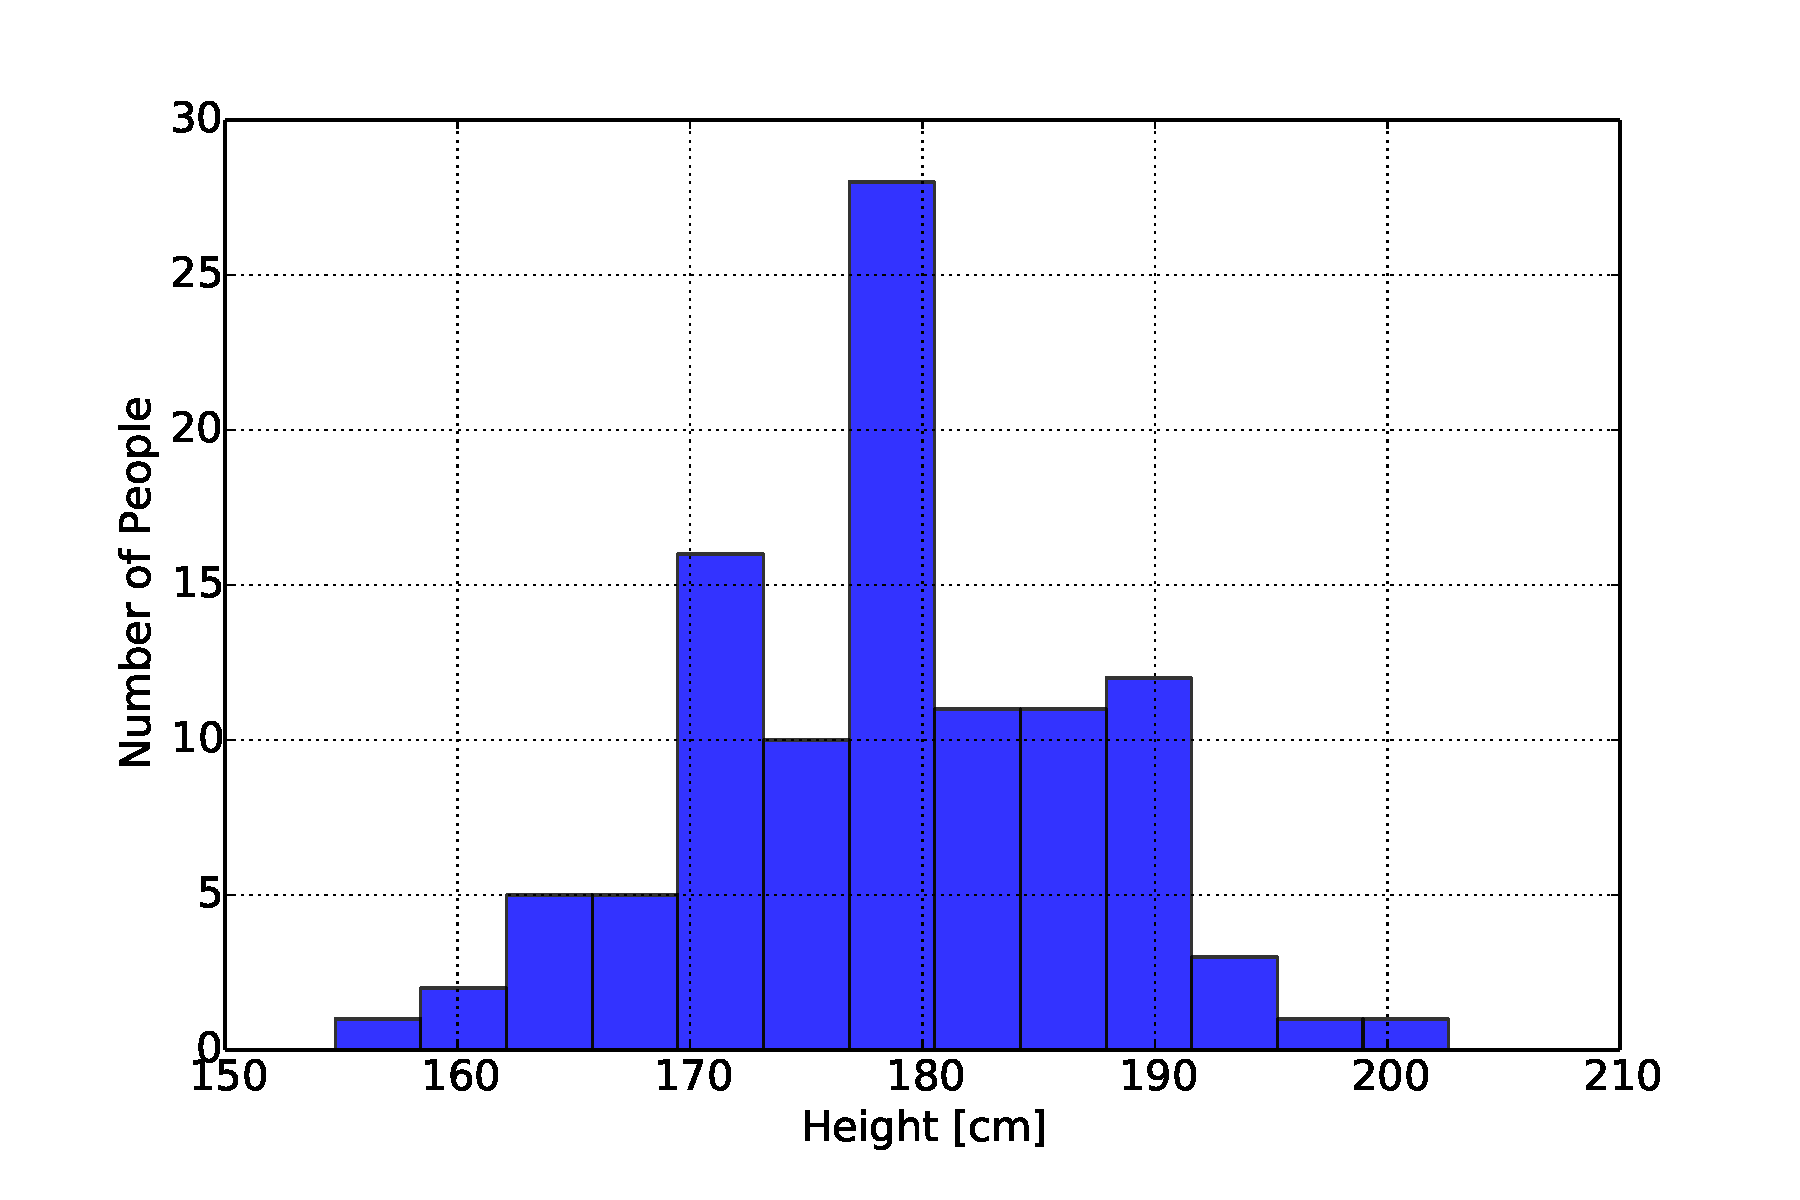
\includegraphics{histmale}
From this histogram, we can immediately observe several quantities which summarize their data:
\be
\i The {\em average value} (around the middle) should be around 175 cm.  The actual value can be calculated from the data, as 
\beqn
\bar{x} &=& \frac{177.8 + 160.0 + \cdots + 180.34 + 183.0}{106} = 178.83
\eeqn
\i The {\em range} of the data is around 155 cm up to about 205 cm.  Again we can be more precise, and find the minimum of the data (154.94 cm) and the maximum (200 cm) but the histogram picture yields an approximate value instantly.
\i The values are {\em roughly symmetric} about the mean (i.e. average) value.  This can give us a clue concerning how to model the data.
\ee
What is quite clear is that it is far easier to deal with a histogram, as above, than find the same information from the table of numbers.

\paragraph{Too Few Bins}

Plotting the same histogram with too few bins might look like:

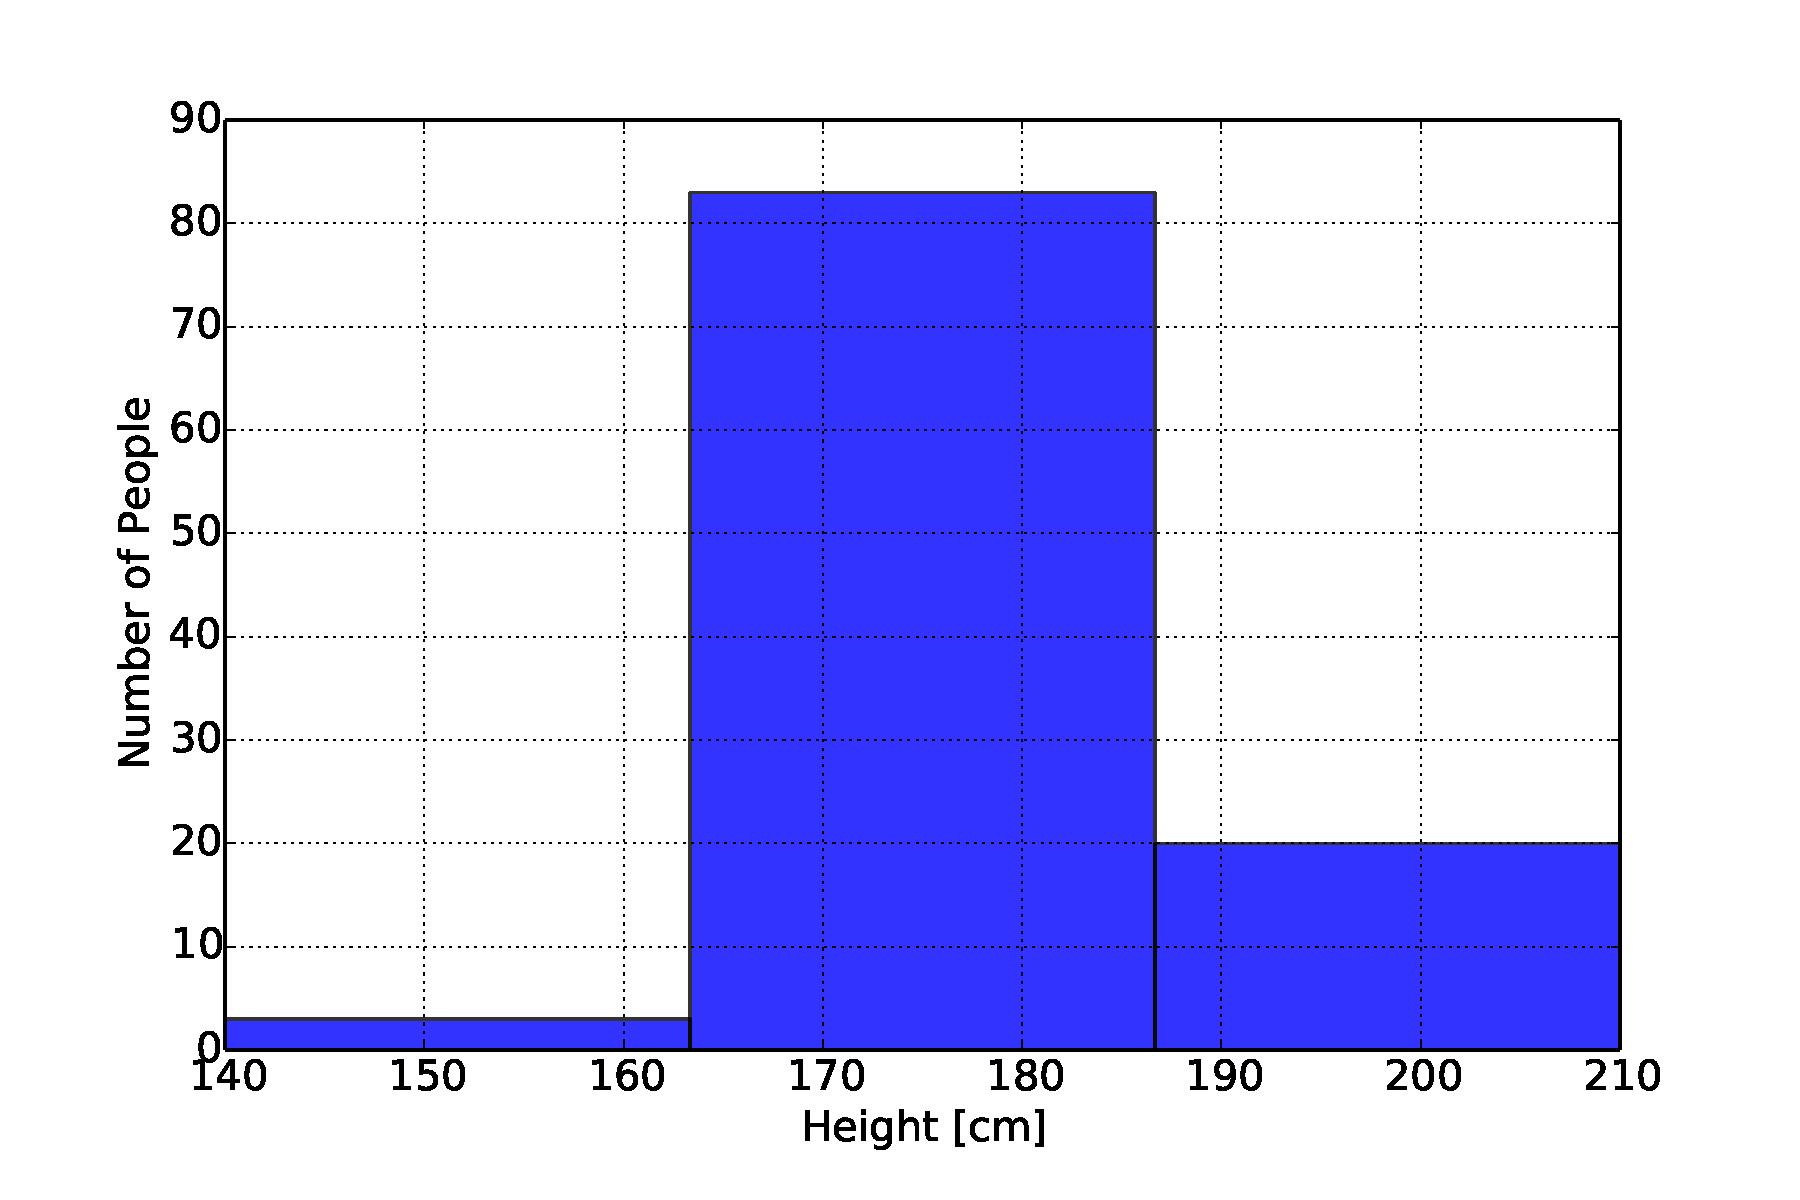
\includegraphics{histmale_toofewbins}

Clearly all the information is washed out.

\paragraph{Too Many Bins}

Plotting the same histogram with too many bins might look like:

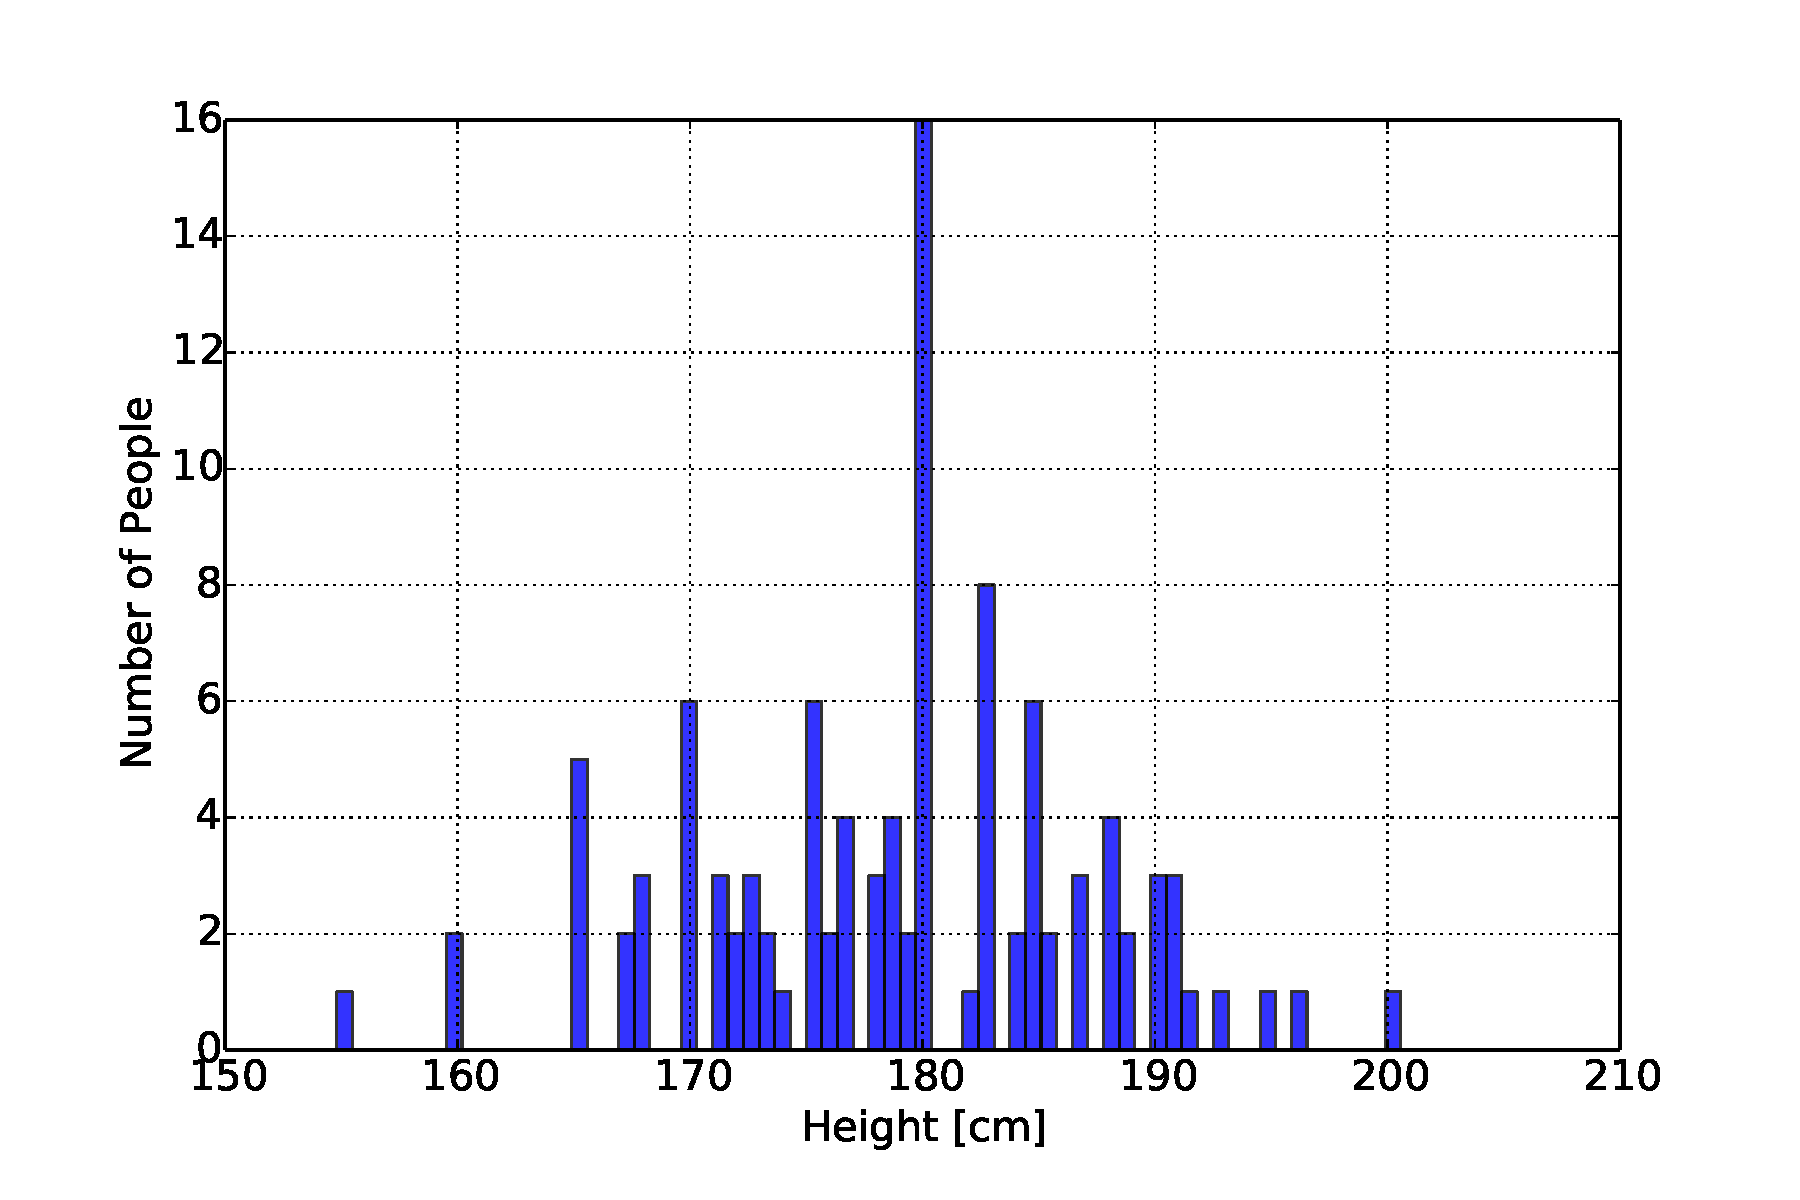
\includegraphics{histmale_toomanybins}

We lose any of the summary information here, where we essentially have one bar for each data-point.


\subsection{Scatter Plots}

A {\em scatter plot} is used to explore the relationship between two values.  For example, in the survey of male students, in addition to height the students also measured the width of their writing hand viewed as a histogram, here

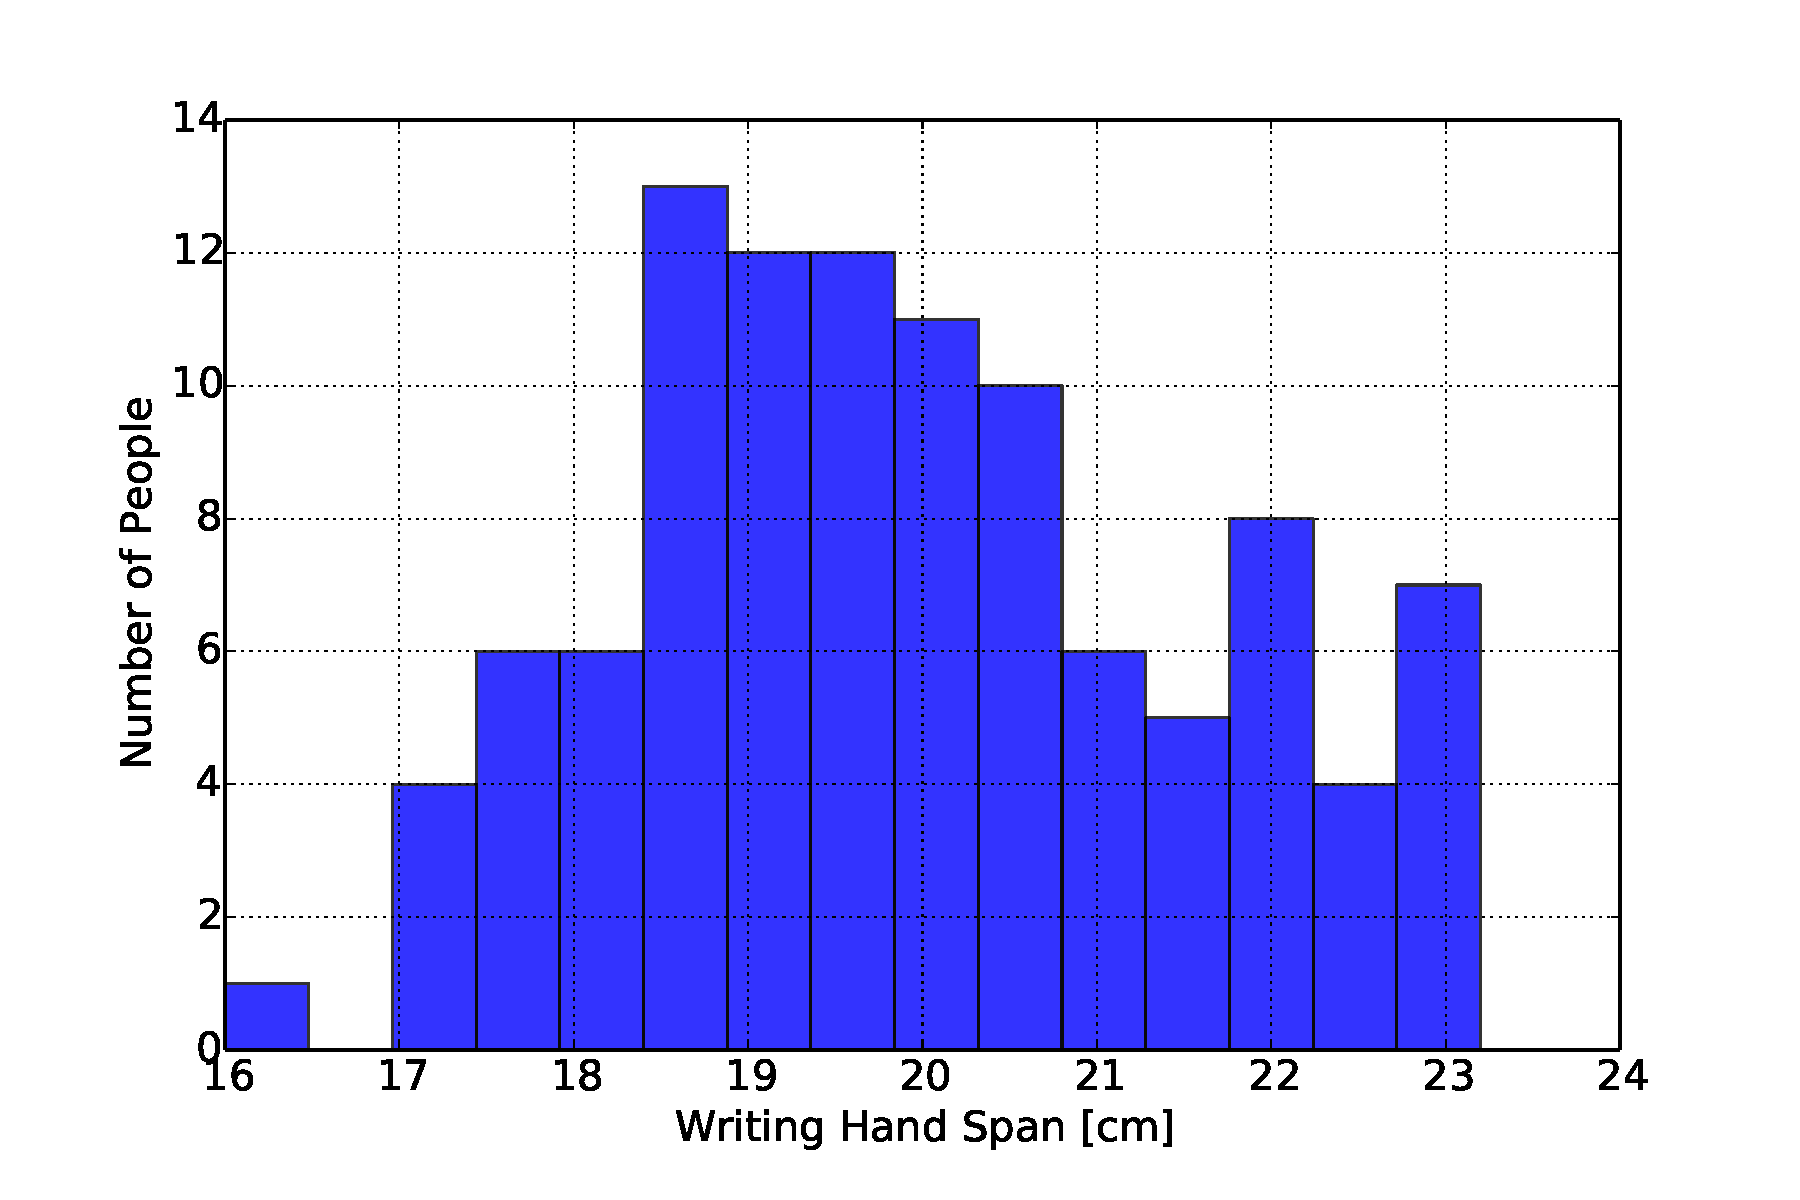
\includegraphics{wrhand_hist}

However, due to the possibility that these two variables could be {\em related}, it makes more sense to make a scatter plot.  In such a plot, one designates one variable as ``x'' and another as ``y,'' and places a {\em single dot} for each pair of values in the data set.  Thus, each dot on the plot corresponds to height and hand-width for a \emph{single} student. 

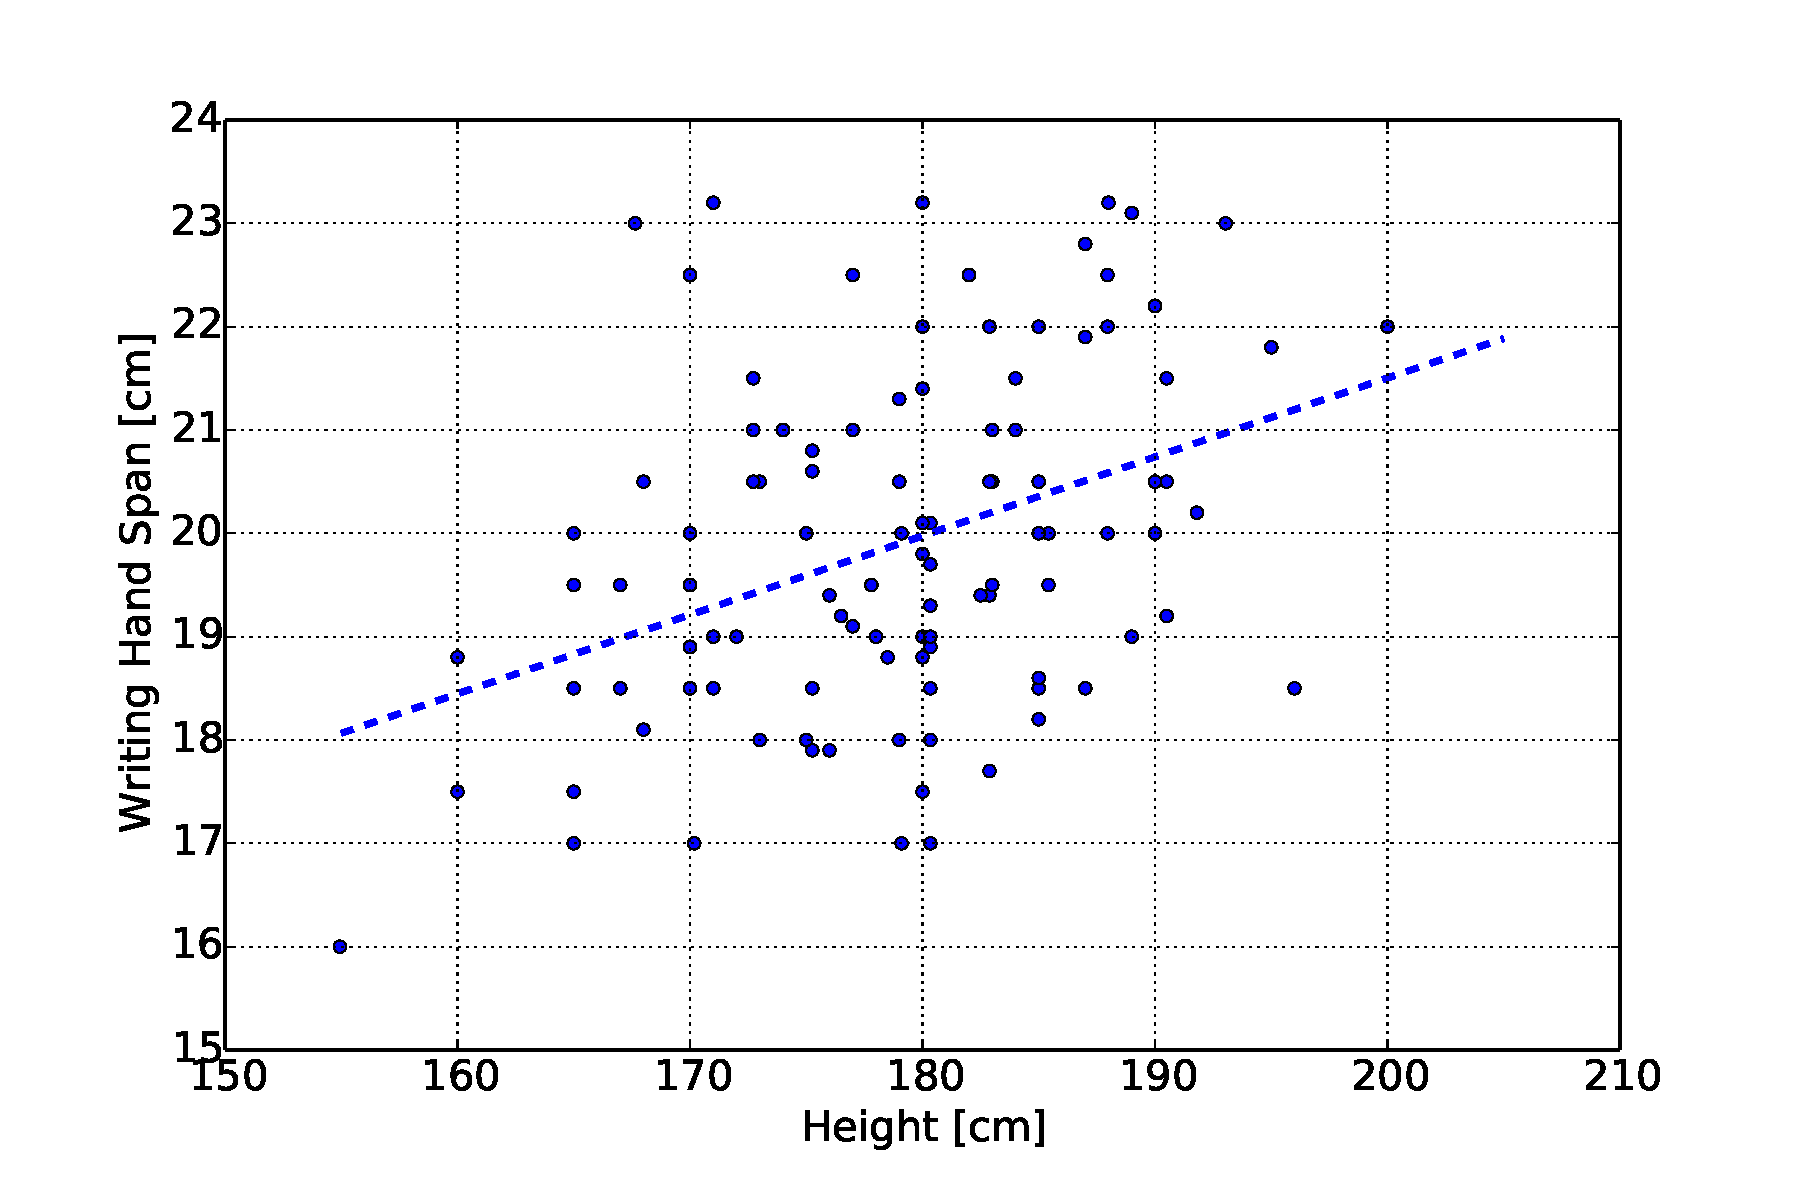
\includegraphics{height_wrhand_scatter}

What we can see here, which was obscured with a histogram, is the {\em relationship} between these values - for the taller students, their hands are wider. We will explore quantifying this relationship later, but much can be done by eye using a scatter plot.


\section{Computer Examples}

This section summarizes how to make histograms and scatter plots with the computer software.

\begin{fullwidth}
\subsection{Histograms}


\begin{lstlisting}
from sie import *
\end{lstlisting}

Load a sample data set, and select only the Male data...

\begin{lstlisting}
data=load_data('data/survey.csv')
male_data=data[data['Sex']=='Male']
\end{lstlisting}

select only the height data, and drop the missing data (na)...

\begin{lstlisting}
male_height=male_data['Height'].dropna()
\end{lstlisting}

make the histogram

\begin{lstlisting}
hist(male_height,bins=20)
xlabel('Height [cm]')
ylabel('Number of People')
\end{lstlisting}

\begin{verbatim}
<matplotlib.text.Text at 0x1085728d0>
\end{verbatim}

\begin{center}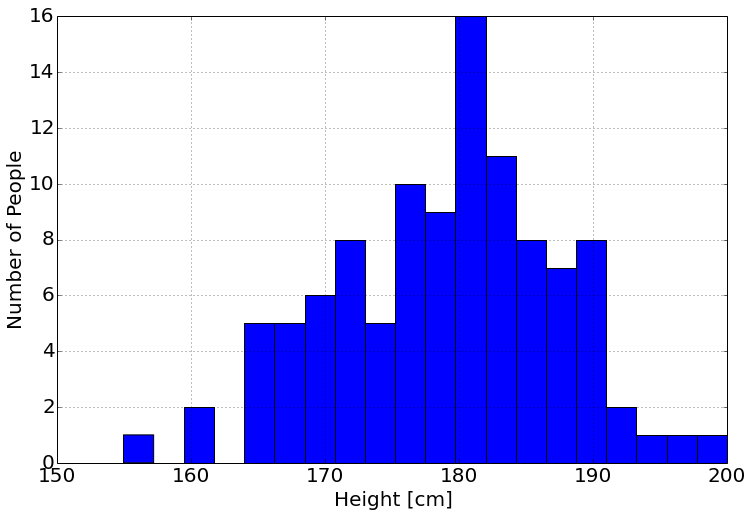
\includegraphics[width=4.5in]{Random_Sequences_and_Visualization/Random_Sequences_and_Visualization_fig0.png}\end{center}

\subsection{Scatter Plot}


\begin{lstlisting}
from sie import *
\end{lstlisting}

Load a sample data set, and select only the Male data...

\begin{lstlisting}
data=load_data('data/survey.csv')
male_data=data[data['Sex']=='Male']
\end{lstlisting}

select only the height and the width of writing hand data, and drop the missing
data (na)...

\begin{lstlisting}
subdata=male_data[['Height','Wr.Hnd']].dropna()
height=subdata['Height']
wr_hand=subdata['Wr.Hnd']
\end{lstlisting}

plot the data

\begin{lstlisting}
plot(height,wr_hand,'o')
ylabel('Writing Hand Span [cm]')
xlabel('Height [cm]')
\end{lstlisting}

\begin{verbatim}
<matplotlib.text.Text at 0x1085774d0>
\end{verbatim}

\begin{center}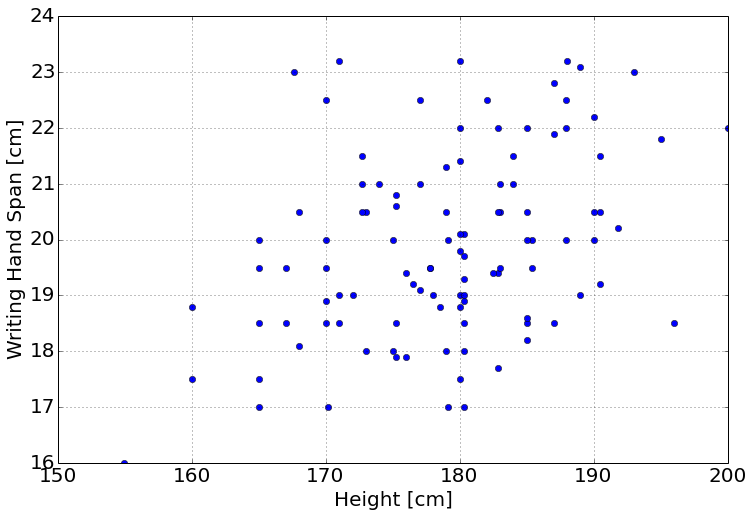
\includegraphics[width=4.5in]{Random_Sequences_and_Visualization/Random_Sequences_and_Visualization_fig1.png}\end{center}


\end{fullwidth}


